\section{UART}
La Unidad de Debug es la encargada de comunicar al pipeline los comandos que recibe por el puerto serial (mediante la UART), asi como de enviar el estado de los latchs del pipeline y los valores de los registros. La UART (Universal Asynchronous Receiver-Transmitter) se encarga de la comunicacion de entrada (RX) y salida (TX), utilizando un generador de baudios para realizar las mismas a una velocidad de 9600 bps.

\subsection{Introducción}
La unidad de debug tiene como entradas:

\begin{itemize}
  \item \textbf{top_clk}: Entrada de clock que se mapea al clock de la FPGA (100 MHz). 
  \item \textbf{rx_done_tick}: Señal que se pone en 1 cuando un dato es recibido en el RX.
  \item \textbf{rx_bus}: Dato recibido por RX.
  \item \textbf{tx_done_tick}: Señal que se pone en 1 cuando un dato es enviado por TX.
  \item \textbf{instruccion}: La instruccion que esta por entrar al latch if-id.
  \item \textbf{send_data}: Datos a ser enviados por TX.
\end{itemize} 

La etapa tiene como salidas:
	 output wire [7:0] tx_bus
\begin{itemize}
	\item \textbf{clk_pipe}: La señal que se utiliza de clock para el pipeline. 
	\item \textbf{rst_pipe}: La señal que se utiliza de reset para el pipeline.
	\item \textbf{tx_start}: Señal que da comienzo al envio de 1 byte por TX. 
	\item \textbf{tx_bus}: El byte que se enviara por TX.
\end{itemize} 

\begin{figure}[H]
\centering
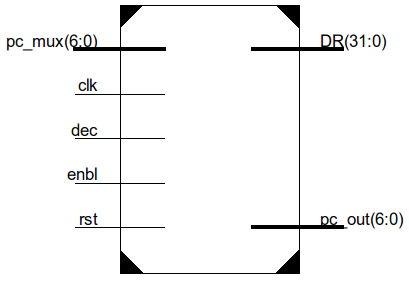
\includegraphics[scale=0.35]{Capitulo01/fetchstage}
\caption{Etapa de búsqueda}
\label{fig:fetch}
\end{figure}

\subsection{Funcionamiento}
La unidad de debug funciona con una maquina de nueve estados. Cabe destacar que para el funcionamiento de los envios, se asigna al tx_bus el primer byte de un registro local llamado buffer. La maquina de estados tiene los siguientes estados:
\begin{itemize}
	\item \textbf{IDLE}: Es el estado inicial. En el mismo se espera la llegada de uno de tres comandos disponibles por RX. Los comandos son S (step), C (continue), R (reset). 
	\item \textbf{STEP}: El comando S nos lleva al estado STEP1. La combinacion de este estado con el estado STEP2 da un ciclo de reloj al pipeline mediante la señal clk_pipe. Por ultimo, el estado STEP2 realiza una copia de los datos del bus send_data en el registro local buffer y nos lleva al estado SEND1.
	\item \textbf{CONT}: El comando C nos lleva al estado CONT1. En este estado se chequea que las instrucciones que estan saliendo de la etapa instruction fetch sean NOP's. Si se dan 4 instrucciones NOP seguidas, se procede a realizar una copia de los datos del bus send_data en el registro local buffer y saltar al estado SEND1. Mientras no sean 4 instrucciones NOP, se salta al estado CONT2, que en combinacion con el estado CONT3 dan un ciclo de reloj al pipeline mediante la señal clk_pipe.
	\item \textbf{RESET}: El comando R nos lleva al estado RESET. Al acceder a este estado se resetea el pipeline mediante la señal rst_pipe y se vuelve al estado IDLE.
	\item \textbf{SEND}: En el estado SEND1 se envia el primer byte del buffer levantando la señal tx_start, y luego se pasa al estado SEND2. En este ultimo estado, se realiza un shift hacia la derecha de 8 bits del buffer y se envia nuevamente el primer byte del buffer. Esta accion se realiza hasta enviar todos los datos, para luego volver al estado IDLE.
\end{itemize} 

\subsection{RX}
La unidad RX es la utilizada para recibir datos por el puerto serial de la FPGA. La placa proporciona el pin N17 por el cual entran los datos serializados, y se trabaja con un tick que sale del generador de baudios para muestrear la señal.
El modulo funciona con una maquina de estados. En un comienzo se esta esperando la llegada de un bit de comienzo. Al detectarlo se pasa al siguiente estado. En este estado se muestrea la señal en su punto medio, guardando el valor del primer bit. Esto se hace para los 8 bits. Por ultimo se detectan los bit de parada, terminando la recepcion de un dato y volviendo al primer estado.  

\subsection{TX}
La unidad TX es la utilizada para enviar datos por el puerto serial de la FPGA. La placa proporciona el pin N18 por el cual entran los datos serializados, y se trabaja con un tick que sale del generador de baudios para respetar el tiempo que el cada bit debe mantenerse para que el receptor que esta escuchando pueda muestrear la señal correcta.
El modulo funciona con una maquina de estados. En un comienzo se esta esperando que la señal tx_start se levante. Al detectar esto se realiza una copia de los datos a enviar y se pasa al siguiente estado. Se realiza el envio serial del byte completo y por ultimo se envian los bit de parada, terminando asi el envio de un dato y volviendo al primer estado.  


\subsection{Generador de Baudios}
El Generador de Baudios genera una señal con una frecuencia menor a la del clock. Para hacer esto tiene un contador que al alcanzar un valor limite levanta la señal de tick. El limite se calcula con la siguiente formula: FrecClk/(BaudRate*16) donde la FrecClk = 100 MHz y el Baud Rate es 9600.